\documentclass[crop, tikz]{standalone}
\usepackage{tikz}
\usepackage{pgfplots}

\usetikzlibrary{arrows,shapes, decorations.pathmorphing,backgrounds,positioning}
\usetikzlibrary{decorations.pathreplacing}
\usetikzlibrary{arrows.meta}

\tikzstyle{smallinvis}=[line width=0mm, fill=white, outer sep=0pt, inner sep=0pt]


\begin{document}
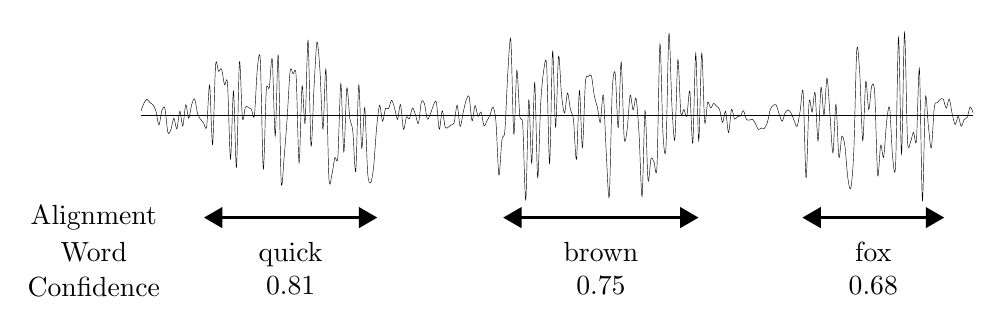
\begin{tikzpicture}[scale=0.4, samples=280, domain=0:7*360]
    \begin{axis}[
        width=28cm, height=8cm,
        enlarge x limits=false,
        xtick=\empty,
        axis lines*=middle,
        hide y axis
    ]
    \addplot [no markers, smooth] { (sin(3*x)+rand*2) * (x < 200) + (3*sin(3*x)+rand*10) * and(x > 200, x < 720) + (sin(3*x)+rand*2) * and(x > 720, x < 1080) + (3*sin(3*x)+rand*10) * and(x > 1080, x < 1700) + (sin(3*x)+rand*2) * and(x > 1700, x < 2000) + (3*sin(3*x)+rand*10) * and(x > 2000, x < 2400) + (sin(3*x)+rand*2) * (x > 2400)};
    \end{axis}
    \node[smallinvis] (i1) at (-1.5, 0) {Alignment};
    \node[smallinvis] (i2) at (-1.5, -1.1) {Word};
    \node[smallinvis] (i3) at (-1.5, -2.2) {Confidence};

    \draw[>=triangle 60, thick, <->, align=center] (2,0) -- node [midway, below] {\\ quick \\ 0.81} (7.5,0);
    \draw[>=triangle 60, thick, <->,  align=center] (11.5,0) -- node [midway, below] {\\ brown \\ 0.75}  (17.7,0);
    \draw[>=triangle 60, thick, <->,  align=center] (21,0) -- node [midway, below] {\\ fox \\ 0.68}  (25.5,0);
\end{tikzpicture}

\end{document}